В \textbf{первой главе} приведены основные понятия теории нечётких множеств и описаны актуальные модели представления нечёткой информации, используемые в дальнейшем при описании исследования. Дано определение нечётких моделей и их классификация в~зависимости от этапа применения нечёткой математики~--- при описании системы, при задании параметров, при задании входов, выходов и состояний (модели первого, второго и третьего типа). В работе предложена классификация нечётких моделей на основе применяемого в них языка описания выбора, объединённая с вышеописанной (рис.~\ref{fig:choice-classification}). В качестве объекта исследования выбраны модели, использующие чёткие отношения и нечёткие параметры (модели второго типа).
\begin{figure}[h] 
  \center
  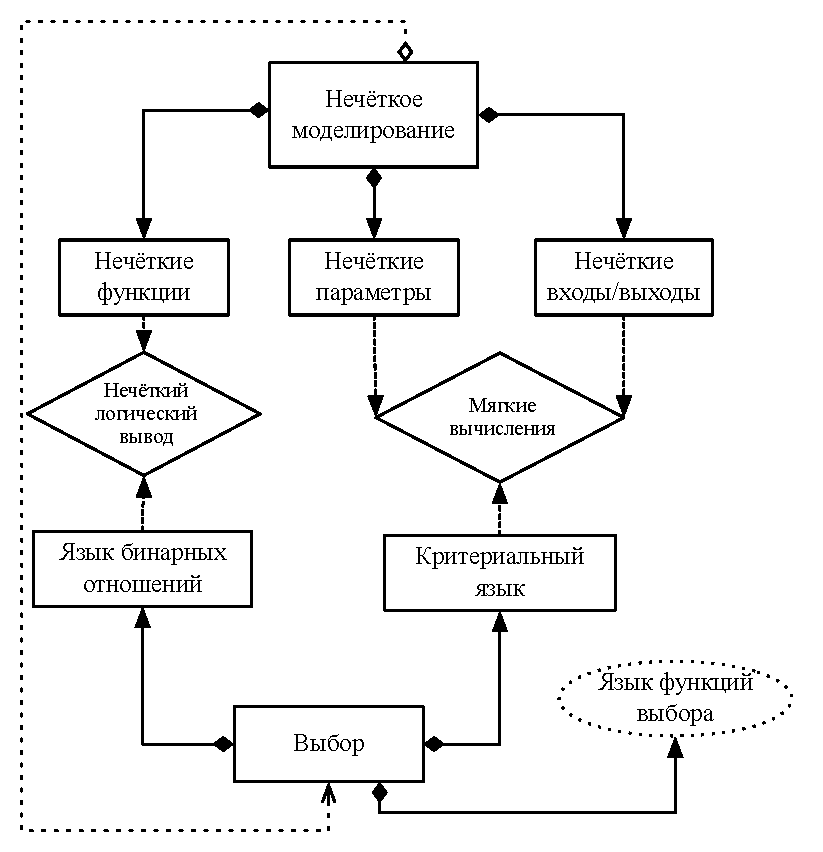
\includegraphics[scale=0.8]{choice-classification}
  \caption{Предлагаемая классификация нечётких моделей} 
  \label{fig:choice-classification}
\end{figure}

Особенностью рассматриваемых моделей является то, что существующие подходы к нечётким вычислениям далеко не всегда применимы в них. Нечёткий логический вывод неадекватен моделям второго типа, поскольку рассчитан на нечёткость отношений, отсутствие формализованных математических моделей либо способов решения с помощью классической теории. Лежащие в основании большинства способов <<мягких вычислений>> алгебраические структуры (в основном решётки) и отсутствие отношения линейного порядка приводят к нарушениям естественных математических отношений и неоправданному расширению неопределённости результата. В диссертации формулируются основные требования к модели представления нечёткой информации и методам решения задач второго типа~--- получение устойчивого решения, непротиворечивость естественным математическим отношениям, ограничение расширения неопределенности,~--- и вводятся требования вычислительной эффективности и возможности применения стандартных программных комплексов, предназначенных для чётких вычислений.

\textbf{Вторая глава} диссертации посвящена разработке и исследованию методов моделирования и обработки нечетких числовых величин, которые удовлетворяли бы выдвинутым к ним в главе 1 требованиям. 

В \textbf{третьей главе} происходит тестирование разработанных моделей и методов обработки нечетких числовых величин на примере задачи сетевого планирования с нечёткими временными оценками.

В \textbf{четвертой главе} рассмотрено применение методов, представленных в диссертации, для усовершенствования процесса предварительного планирования проектов по разработке программного обеспечения. Отличительной особенностью таких проектов является наличие нечёткой неопределённости сроков выполнения операций, обусловленной внешними факторами. 

В качестве средства разработки применяется интегрированная среда Microsoft Visual Studio 2010. Особенностью разработанного программного продукта <<CSBusinessGraph>> является то, что он не использует никаких специализированных средств и третьесторонних библиотек для представления нечётких чисели выполняет все вычисления только с использованием действительных переменных.

К основным \textit{функциональным возможностям} программного продукта относятся: создание модели проекта в виде вершинного графа в ручном режиме или импорт существующей модели из XML-файла; поддержка модели проекта в согласованном состоянии~--- проверка отсутствия циклов в графе и наличие только одной компоненты связности; формирование временных оценок выполнения операций, выраженных в~виде треугольных чисел; автоматическое преобразование вершинного графа в~стрелочный; реализация механизма расчёта критического пути на~основе $\alpha$-уровневых и~двухточечных вычислений с применением выбранного пользователем  вида значений параметров $\lambda$ преобразования L; экспорт отчёта о~решении задачи в~формат Microsoft Excel с~формированием графиков для модифицированных нечётких оценок, общего времени выполнения проекта и~построением стрелочного графа c~выделением критических операций.

На рис.~\ref{fig:app-sample-graph} изображено главное окно приложения с открытым в нём проектом.
\begin{figure}[h] 
  \center
  \includegraphics[scale=0.5]{app-sample-graph.png}
  \caption{Главное окно приложения} 
  \label{fig:app-sample-graph}
\end{figure}
